% Options for packages loaded elsewhere
\PassOptionsToPackage{unicode}{hyperref}
\PassOptionsToPackage{hyphens}{url}
%
\documentclass[
  man,floatsintext]{apa6}
\usepackage{amsmath,amssymb}
\usepackage{lmodern}
\usepackage{iftex}
\ifPDFTeX
  \usepackage[T1]{fontenc}
  \usepackage[utf8]{inputenc}
  \usepackage{textcomp} % provide euro and other symbols
\else % if luatex or xetex
  \usepackage{unicode-math}
  \defaultfontfeatures{Scale=MatchLowercase}
  \defaultfontfeatures[\rmfamily]{Ligatures=TeX,Scale=1}
\fi
% Use upquote if available, for straight quotes in verbatim environments
\IfFileExists{upquote.sty}{\usepackage{upquote}}{}
\IfFileExists{microtype.sty}{% use microtype if available
  \usepackage[]{microtype}
  \UseMicrotypeSet[protrusion]{basicmath} % disable protrusion for tt fonts
}{}
\makeatletter
\@ifundefined{KOMAClassName}{% if non-KOMA class
  \IfFileExists{parskip.sty}{%
    \usepackage{parskip}
  }{% else
    \setlength{\parindent}{0pt}
    \setlength{\parskip}{6pt plus 2pt minus 1pt}}
}{% if KOMA class
  \KOMAoptions{parskip=half}}
\makeatother
\usepackage{xcolor}
\IfFileExists{xurl.sty}{\usepackage{xurl}}{} % add URL line breaks if available
\IfFileExists{bookmark.sty}{\usepackage{bookmark}}{\usepackage{hyperref}}
\hypersetup{
  pdftitle={Satisfying housework division? Gender role beliefs and religion as moderators of housework division and satisfaction},
  pdfauthor={Carlotta Reinhardt1, Margaret Bassney1, \& Anushree Goswami1},
  pdflang={en-EN},
  hidelinks,
  pdfcreator={LaTeX via pandoc}}
\urlstyle{same} % disable monospaced font for URLs
\usepackage{graphicx}
\makeatletter
\def\maxwidth{\ifdim\Gin@nat@width>\linewidth\linewidth\else\Gin@nat@width\fi}
\def\maxheight{\ifdim\Gin@nat@height>\textheight\textheight\else\Gin@nat@height\fi}
\makeatother
% Scale images if necessary, so that they will not overflow the page
% margins by default, and it is still possible to overwrite the defaults
% using explicit options in \includegraphics[width, height, ...]{}
\setkeys{Gin}{width=\maxwidth,height=\maxheight,keepaspectratio}
% Set default figure placement to htbp
\makeatletter
\def\fps@figure{htbp}
\makeatother
\setlength{\emergencystretch}{3em} % prevent overfull lines
\providecommand{\tightlist}{%
  \setlength{\itemsep}{0pt}\setlength{\parskip}{0pt}}
\setcounter{secnumdepth}{-\maxdimen} % remove section numbering
% Make \paragraph and \subparagraph free-standing
\ifx\paragraph\undefined\else
  \let\oldparagraph\paragraph
  \renewcommand{\paragraph}[1]{\oldparagraph{#1}\mbox{}}
\fi
\ifx\subparagraph\undefined\else
  \let\oldsubparagraph\subparagraph
  \renewcommand{\subparagraph}[1]{\oldsubparagraph{#1}\mbox{}}
\fi
\newlength{\cslhangindent}
\setlength{\cslhangindent}{1.5em}
\newlength{\csllabelwidth}
\setlength{\csllabelwidth}{3em}
\newlength{\cslentryspacingunit} % times entry-spacing
\setlength{\cslentryspacingunit}{\parskip}
\newenvironment{CSLReferences}[2] % #1 hanging-ident, #2 entry spacing
 {% don't indent paragraphs
  \setlength{\parindent}{0pt}
  % turn on hanging indent if param 1 is 1
  \ifodd #1
  \let\oldpar\par
  \def\par{\hangindent=\cslhangindent\oldpar}
  \fi
  % set entry spacing
  \setlength{\parskip}{#2\cslentryspacingunit}
 }%
 {}
\usepackage{calc}
\newcommand{\CSLBlock}[1]{#1\hfill\break}
\newcommand{\CSLLeftMargin}[1]{\parbox[t]{\csllabelwidth}{#1}}
\newcommand{\CSLRightInline}[1]{\parbox[t]{\linewidth - \csllabelwidth}{#1}\break}
\newcommand{\CSLIndent}[1]{\hspace{\cslhangindent}#1}
\ifLuaTeX
\usepackage[bidi=basic]{babel}
\else
\usepackage[bidi=default]{babel}
\fi
\babelprovide[main,import]{english}
% get rid of language-specific shorthands (see #6817):
\let\LanguageShortHands\languageshorthands
\def\languageshorthands#1{}
% Manuscript styling
\usepackage{upgreek}
\captionsetup{font=singlespacing,justification=justified}

% Table formatting
\usepackage{longtable}
\usepackage{lscape}
% \usepackage[counterclockwise]{rotating}   % Landscape page setup for large tables
\usepackage{multirow}		% Table styling
\usepackage{tabularx}		% Control Column width
\usepackage[flushleft]{threeparttable}	% Allows for three part tables with a specified notes section
\usepackage{threeparttablex}            % Lets threeparttable work with longtable

% Create new environments so endfloat can handle them
% \newenvironment{ltable}
%   {\begin{landscape}\centering\begin{threeparttable}}
%   {\end{threeparttable}\end{landscape}}
\newenvironment{lltable}{\begin{landscape}\centering\begin{ThreePartTable}}{\end{ThreePartTable}\end{landscape}}

% Enables adjusting longtable caption width to table width
% Solution found at http://golatex.de/longtable-mit-caption-so-breit-wie-die-tabelle-t15767.html
\makeatletter
\newcommand\LastLTentrywidth{1em}
\newlength\longtablewidth
\setlength{\longtablewidth}{1in}
\newcommand{\getlongtablewidth}{\begingroup \ifcsname LT@\roman{LT@tables}\endcsname \global\longtablewidth=0pt \renewcommand{\LT@entry}[2]{\global\advance\longtablewidth by ##2\relax\gdef\LastLTentrywidth{##2}}\@nameuse{LT@\roman{LT@tables}} \fi \endgroup}

% \setlength{\parindent}{0.5in}
% \setlength{\parskip}{0pt plus 0pt minus 0pt}

% Overwrite redefinition of paragraph and subparagraph by the default LaTeX template
% See https://github.com/crsh/papaja/issues/292
\makeatletter
\renewcommand{\paragraph}{\@startsection{paragraph}{4}{\parindent}%
  {0\baselineskip \@plus 0.2ex \@minus 0.2ex}%
  {-1em}%
  {\normalfont\normalsize\bfseries\itshape\typesectitle}}

\renewcommand{\subparagraph}[1]{\@startsection{subparagraph}{5}{1em}%
  {0\baselineskip \@plus 0.2ex \@minus 0.2ex}%
  {-\z@\relax}%
  {\normalfont\normalsize\itshape\hspace{\parindent}{#1}\textit{\addperi}}{\relax}}
\makeatother

% \usepackage{etoolbox}
\makeatletter
\patchcmd{\HyOrg@maketitle}
  {\section{\normalfont\normalsize\abstractname}}
  {\section*{\normalfont\normalsize\abstractname}}
  {}{\typeout{Failed to patch abstract.}}
\patchcmd{\HyOrg@maketitle}
  {\section{\protect\normalfont{\@title}}}
  {\section*{\protect\normalfont{\@title}}}
  {}{\typeout{Failed to patch title.}}
\makeatother

\usepackage{xpatch}
\makeatletter
\xapptocmd\appendix
  {\xapptocmd\section
    {\addcontentsline{toc}{section}{\appendixname\ifoneappendix\else~\theappendix\fi\\: #1}}
    {}{\InnerPatchFailed}%
  }
{}{\PatchFailed}
\usepackage{lineno}

\linenumbers
\usepackage{csquotes}
\usepackage[titles]{tocloft}
\cftpagenumbersoff{figure}
\renewcommand{\cftfigpresnum}{\itshape\figurename\enspace}
\renewcommand{\cftfigaftersnum}{.\space}
\setlength{\cftfigindent}{0pt}
\setlength{\cftafterloftitleskip}{0pt}
\settowidth{\cftfignumwidth}{Figure 10.\qquad}
\cftpagenumbersoff{table}
\renewcommand{\cfttabpresnum}{\itshape\tablename\enspace}
\renewcommand{\cfttabaftersnum}{.\space}
\setlength{\cfttabindent}{0pt}
\setlength{\cftafterloftitleskip}{0pt}
\settowidth{\cfttabnumwidth}{Table 10.\qquad}
\ifLuaTeX
  \usepackage{selnolig}  % disable illegal ligatures
\fi

\title{Satisfying housework division? Gender role beliefs and religion as moderators of housework division and satisfaction}
\author{Carlotta Reinhardt\textsuperscript{1}, Margaret Bassney\textsuperscript{1}, \& Anushree Goswami\textsuperscript{1}}
\date{}


\shorttitle{gender roles, housework and satisfaction}

\affiliation{\vspace{0.5cm}\textsuperscript{1} Smith College}

\begin{document}
\maketitle

\hypertarget{results}{%
\section{Results}\label{results}}

\hypertarget{analysis-strategy}{%
\subsection{Analysis Strategy}\label{analysis-strategy}}

To test our hypotheses that gender role beliefs and religion moderate the relationship between housework distribution and satisfaction, we used multilevel modeling and the Actor-Partner Interdependence Model (Kenny, Kashy, \& Cook, 2020). The APIM measures the effect of the explanatory variables for both members in a dyad at the same time, so actor as well as partner effects could be considered in our analysis. This way, it is possible to see how one partner's housework distribution affects both their own satisfaction with the housework distribution (actor effect) and their partner's satisfaction with the housework distribution (partner effect). In this analysis, we will look at the moderating effect of each partner's gender role beliefs on the two actor effects (shown in figure 1) as well as on the partner effects.Our research studied people in relationships, where each pair in a relationship is refered to as a dyad. Since we were working with dyadic data, our data was not independent. For example the amount of housework one partner does, will be correlated with how much housework the other partner does.This will result in correlated residuals. To account for the nonindependence, the APIM considered how much of the variation in satisfaction was caused by the dyad compared to housework distribution and gender role beleifs. To account for the correlated errors, we weighted each dyad so that the residuals of each individual were constant.



\begin{figure}
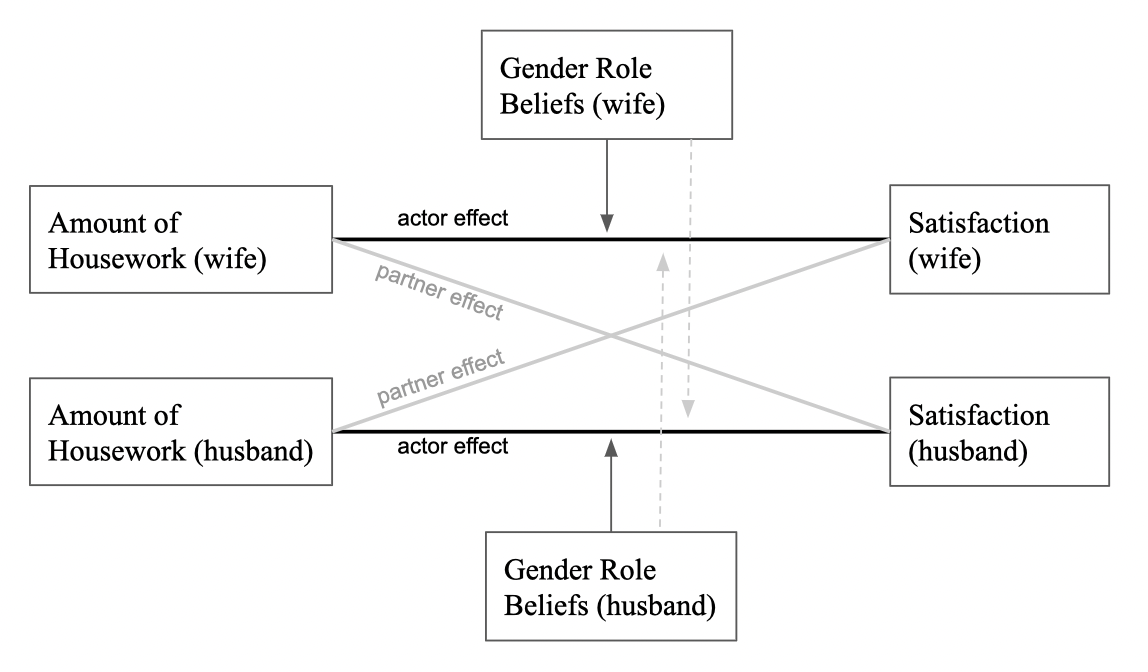
\includegraphics[width=3.83in]{APIM} \caption{Schematic representation of actor and partner effects in the APIM moderated by gender role beliefs.}\label{fig:unnamed-chunk-3}
\end{figure}

\hypertarget{main-results}{%
\subsection{Main Results}\label{main-results}}

\hypertarget{gender-role-beliefs}{%
\paragraph{Gender Role Beliefs}\label{gender-role-beliefs}}

All relevant results of the moderation analysis in the APIM are shown in figure 2. It was shown that for husbands and wives, a higher amount of housework was significantly related to a lower satisfaction. For wives we found \(\beta\) =-0.02, \emph{p} = 0.02, and SE =0.01. For husbands we found \(\beta\) =-0.03, \emph{p} = 0.01 and SE = 0.01.
For the female partners, their own gender role beliefs significantly moderated the relationship between their housework distribution and their satisfaction with the housework distribution. The moderation effect was 0.07 (\emph{p} = \textless0.01, SE = 0.02). When the wives had higher gender role beliefs, which means more conservative, their satisfaction with the housework distribution tended to be higher, while keeping their own housework distribution constant at the mean. The husband's gender role beliefs significantly moderated the relationship between the wife's housework distribution and the wife's satisfaction with the housework distribution. The moderation effect was -0.06 (\emph{p} = 0.01, SE = 0.02). When the husbands had more conservative gender role beliefs, the wife's satisfaction decreased by -0.06 while keeping the wives housework distribution constant at the mean. Moreover, a marginally significant moderation effect was found for the relationship between the husbands amount of housework and the wife's satisfaction which was moderated by the wife's gender role beliefs (\(\beta\) = 0.03, \emph{p} =0.10, SE = 0.02). When wives had more conservative gender role beliefs, their satisfaction tended to be higher, while their husbands housework distribution was held constant at the mean.




\begin{figure}
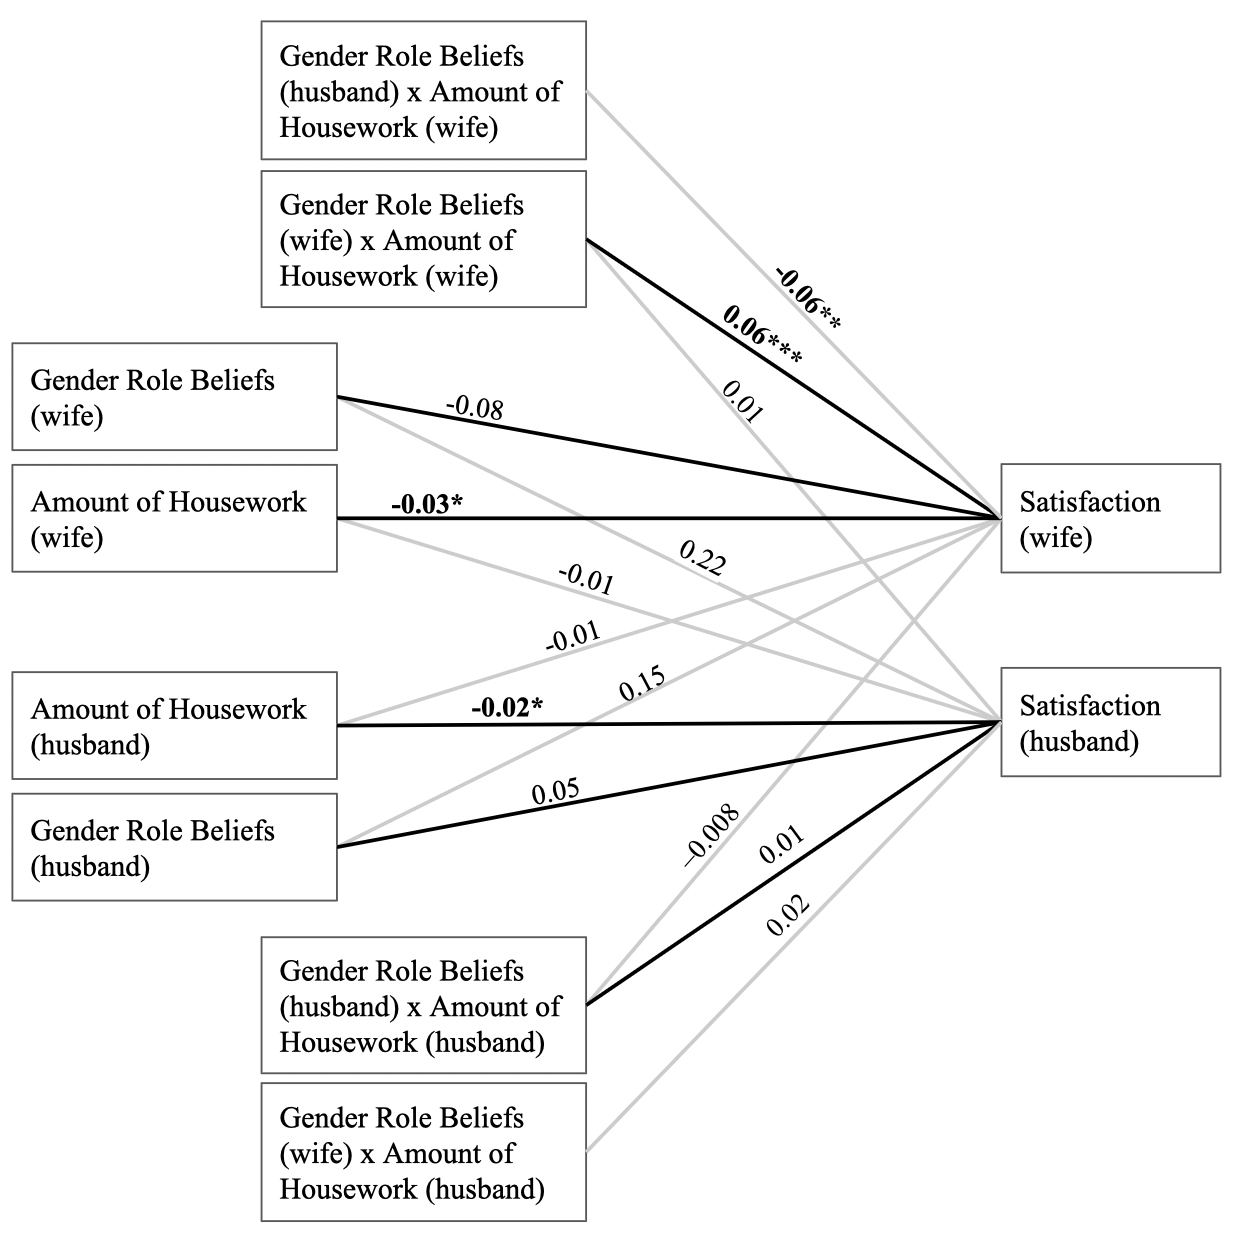
\includegraphics[width=4.11in]{moderation} \caption{Moderation effects in the APIM. Values shown in the figure are \(\beta\) coefficients.
* \emph{p} \textless{} .05, ** \emph{p} \textless{} .01, *** \emph{p} \textless{} .001.}\label{fig:unnamed-chunk-9}
\end{figure}



\begin{figure}
\centering
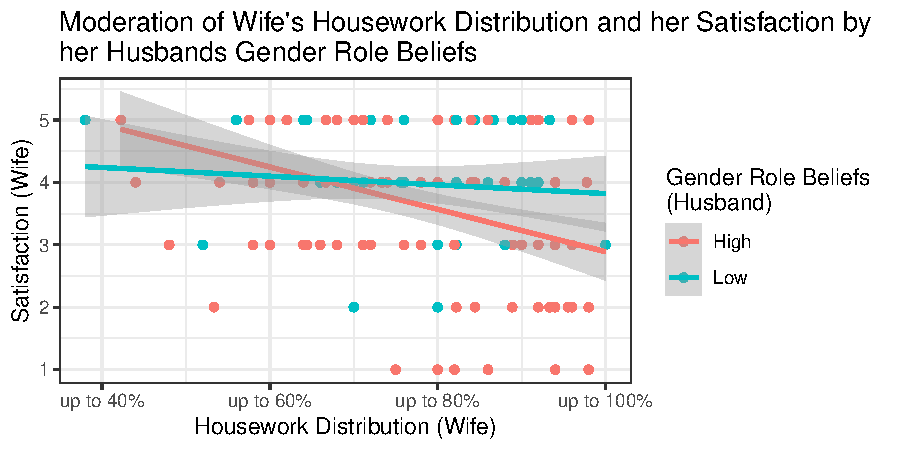
\includegraphics{results_files/figure-latex/unnamed-chunk-12-1.pdf}
\caption{\label{fig:unnamed-chunk-12}Moderation of wife's housework distribution and satisfaction by gender role beliefs. Housework distribution in \%, Satisfaction and gender role beliefs were measured with a 5 point Likert scale (1 = liberal, 5 = conservative).}
\end{figure}



\begin{figure}
\centering
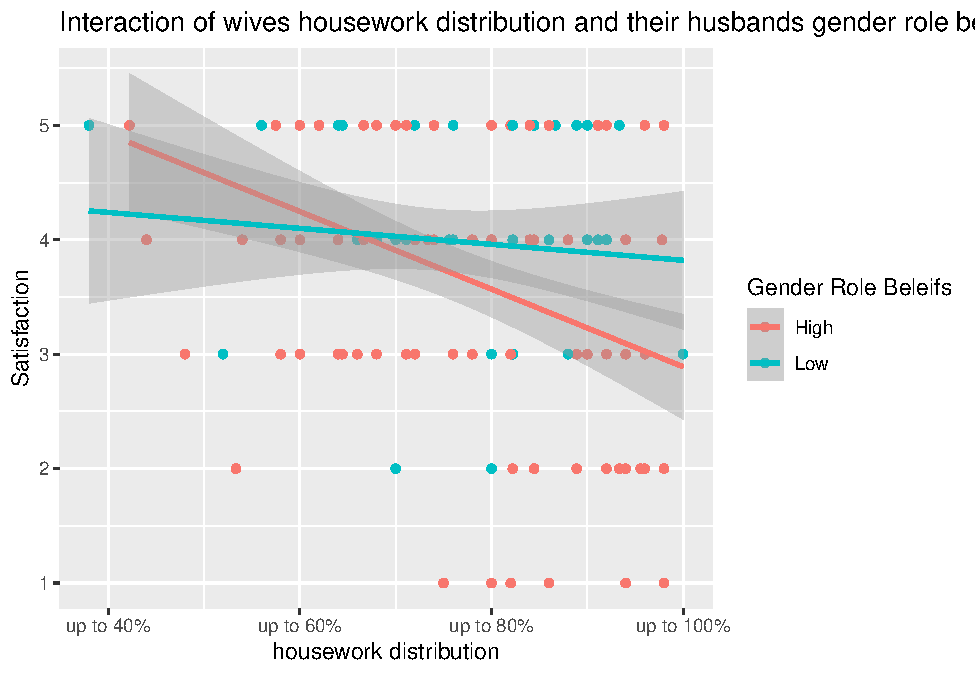
\includegraphics{results_files/figure-latex/unnamed-chunk-13-1.pdf}
\caption{\label{fig:unnamed-chunk-13}Moderation of wife's housework distribution and her satisfaction by their husbands gender role beliefs. Housework distribution in \%, Satisfaction and gender role beliefs were measured with a 5 point Likert scale (1 = liberal, 5 = conservative).}
\end{figure}

Wives who have low gender role beliefs, which means they are more liberal, reported a lower satisfaction with an increasing amount of housework they had to do. Women with more conservative gender role beliefs (high value) did not show a significant decrease in satisfaction with an increasing amount of housework (figure 3).

As the the amount of housework increases for wives whose husbands have low gender role beliefs, their satisfaction remains constant. When housework increases for wives whose husbands have high gender role beliefs, their satisfaction decreases (figure 4).
Since we used distinguishable dyads, gender was a built in moderator. To see if the moderation effects differed significantly by gender, we looked at the three way interactions between gender, housework distribution, and gender role beliefs. We found two significant gender differences in the moderation effects. The interaction between the actor's housework and their own gender role beliefs was significantly different for husbands and wives with an estimate of 0.06 (\emph{p} = 0.03, SE = 0.03). The moderation effect of ones own gender role beliefs was 0.06 units higher for women than men, meaning the moderation effect of gender role beliefs had a significantly larger positive effect on satisfaction for wives than for husbands.
In addition, the interaction between the actor's amount of housework and their partners gender role beliefs was significantly different for husbands and wives with an estimate of -0.08(\emph{p} = 0.01, SE = 0.03).The moderation effect of the partners gender role beliefs was -0.08 units lower for women than men which means that the moderation effect of the husbands gender role beliefs had a significantly larger negative effect on satisfaction compared to how the wifes gender role beliefs effected the relationship between housework distribution and satisfaction for her husband.

\hypertarget{religion}{%
\paragraph{Religion}\label{religion}}

No significant relationships between any of the variables have been found in the APIM model including the moderator religion (\emph{p} \textgreater{} 0.19). Religion did therefore not moderate the relationship between housework distribution and satisfaction for wives and husbands.

\hypertarget{exploratory-results}{%
\subsection{Exploratory Results}\label{exploratory-results}}

In order to being able to find possible explanations for the association between gender role beliefs and satisfaction that we found in our analysis, we conducted a simple mediation analysis, investigating whether the wife's gatekeeping mediated the relationship between her gender role beliefs and her satisfaction, and therefore could explain the patterns found in the prior analysis. Are women with higher gender role beliefs more likely to gatekeep housework tasks which would in turn lead to a higher satisfaction?
Linear models will be calculated for all paths to see whether all paths are significant first, before we will calculate the mediation effect in a second step.




\begin{figure}
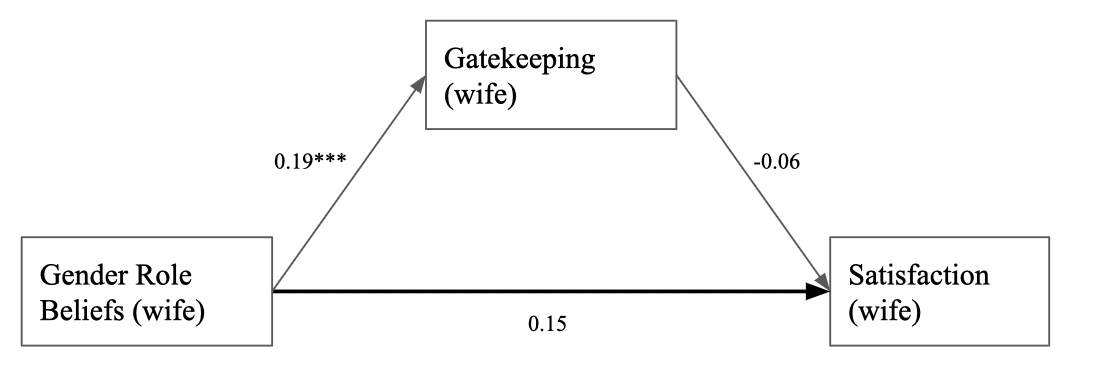
\includegraphics[width=3.69in]{mediation} \caption{Proposed mediation model with wife's gatekeeping as the mediator of the wife's gender role beliefs and satisfaction. Values shown in the figure are \(\beta\) coefficients.
* \emph{p} \textless{} .05, ** \emph{p} \textless{} .01, *** \emph{p} \textless{} .001.}\label{fig:unnamed-chunk-19}
\end{figure}

As seen in figure 5, no significant relationship between gender role beliefs and satisfaction has been found, despite the moderating effect of gender role beliefs that has been found before.

\hypertarget{references}{%
\section{References}\label{references}}

\hypertarget{refs}{}
\begin{CSLReferences}{1}{0}
\leavevmode\vadjust pre{\hypertarget{ref-kenny2020dyadic}{}}%
Kenny, D. A., Kashy, D. A., \& Cook, W. L. (2020). \emph{Dyadic data analysis}. Guilford Publications.

\end{CSLReferences}


\clearpage
\renewcommand{\listfigurename}{Figure captions}

\clearpage
\renewcommand{\listtablename}{Table captions}


\end{document}
